\documentclass[11pt,a4paper]{article}

% ─── Encoding & fonts ────────────────────────────────────────────────────────
\usepackage[T1]{fontenc}
\usepackage[utf8]{inputenc}
\usepackage{lmodern}
\usepackage{microtype}

% ─── Layout ──────────────────────────────────────────────────────────────────
\usepackage[a4paper,margin=1in]{geometry}
\usepackage{graphicx}
\usepackage{booktabs}
\usepackage{tabularx}
\usepackage{longtable}
\usepackage{enumitem}
\usepackage{parskip}
\usepackage{fancyhdr}
\usepackage{titlesec}
\usepackage[table]{xcolor}
\usepackage{listings}
\usepackage[most]{tcolorbox}
\usepackage{tikz}
\usetikzlibrary{arrows.meta,positioning,fit,backgrounds,calc,shapes.geometric}
\usepackage{float}

% ─── Brand palette (Finals Buddy) ────────────────────────────────────────────
\definecolor{fbSage}{HTML}{A7C4A0}
\definecolor{fbBrown}{HTML}{34302B}
\definecolor{fbRose}{HTML}{D28C97}
\definecolor{fbCream}{HTML}{ECE6DA}
\definecolor{fbInk}{HTML}{141312}
\definecolor{fbMute}{HTML}{6E685C}

% ─── Diagram styles ──────────────────────────────────────────────────────────
% One shared vocabulary so every figure reads the same way:
%   node     plain component        accent  the thing under discussion
%   store    persistent state       ext     outside this system
%   degrade  a silent-failure path (dashed, warm colour)
\tikzset{
  fbfont/.style={font=\sffamily\scriptsize},
  node/.style={
    fbfont, draw=fbMute, line width=0.6pt, rounded corners=2pt,
    fill=white, align=center, inner sep=4pt, minimum height=8mm},
  accent/.style={
    node, draw=fbSage, line width=1.1pt, fill=fbSage!18},
  store/.style={
    node, draw=fbMute, fill=fbCream, align=center},
  ext/.style={
    node, draw=fbMute, dashed, fill=white},
  degrade/.style={
    node, draw=fbRose, line width=0.9pt, fill=fbRose!12},
  grp/.style={
    draw=fbMute!60, line width=0.5pt, rounded corners=3pt,
    inner sep=7pt, fill=fbCream!40},
  grplabel/.style={fbfont, color=fbMute, font=\sffamily\scriptsize\bfseries},
  flow/.style={-{Stealth[length=4pt]}, draw=fbBrown, line width=0.6pt},
  flowlabel/.style={fbfont, color=fbMute, inner sep=2pt},
  warn/.style={-{Stealth[length=4pt]}, draw=fbRose, line width=0.7pt, dashed},
}
% Caption styling to match the document
\usepackage[font=small,labelfont={bf,color=fbBrown},textfont={color=fbMute}]{caption}

% ─── Hyperlinks ──────────────────────────────────────────────────────────────
\usepackage[colorlinks=true]{hyperref}
\hypersetup{
  linkcolor=fbBrown,
  urlcolor=fbRose,
  citecolor=fbSage,
  pdftitle={Finals Buddy — Technical Documentation},
  pdfauthor={Finals Buddy}
}

% ─── Section styling ─────────────────────────────────────────────────────────
\titleformat{\section}
  {\color{fbBrown}\Large\bfseries}{\color{fbSage}\thesection}{0.7em}{}
\titleformat{\subsection}
  {\color{fbBrown}\large\bfseries}{\color{fbSage}\thesubsection}{0.6em}{}
\titlespacing*{\section}{0pt}{1.6em}{0.6em}

% ─── Code / verbatim style ───────────────────────────────────────────────────
\lstdefinestyle{fb}{
  basicstyle=\ttfamily\small\color{fbInk},
  backgroundcolor=\color{fbCream},
  frame=single,
  framerule=0pt,
  rulecolor=\color{fbCream},
  xleftmargin=0.6em,
  xrightmargin=0.6em,
  aboveskip=1em,
  belowskip=1em,
  breaklines=true,
  columns=fullflexible,
  keepspaces=true,
  showstringspaces=false
}
\lstset{style=fb}

% Inline code helper
\newcommand{\code}[1]{\colorbox{fbCream}{\texttt{\small #1}}}

% ─── Table helper: sage header row ───────────────────────────────────────────
\newcommand{\hdr}[1]{\textcolor{white}{\bfseries #1}}
\newcolumntype{L}{>{\raggedright\arraybackslash}X}

% ─── Header / footer ─────────────────────────────────────────────────────────
\pagestyle{fancy}
\fancyhf{}
\renewcommand{\headrulewidth}{0.4pt}
\renewcommand{\headrule}{\hbox to\headwidth{\color{fbSage}\leaders\hrule height 0.8pt\hfill}}
\fancyhead[L]{\small\color{fbMute}Finals Buddy}
\fancyhead[R]{\small\color{fbMute}Technical Documentation}
\fancyfoot[C]{\small\color{fbMute}\thepage}

\setlength{\arrayrulewidth}{0.3pt}
\arrayrulecolor{fbMute}

\begin{document}

% ─── Title page ──────────────────────────────────────────────────────────────
\begin{titlepage}
\centering
\vspace*{3cm}

\includegraphics[width=0.6\textwidth]{logo.png}\\[2cm]
{\color{fbBrown}\Huge\bfseries Technical Documentation}\\[0.5cm]
{\color{fbMute}\large An AI-powered adaptive finals-prep workspace}\\[1.5cm]
{\color{fbSage}\rule{0.5\textwidth}{2pt}}\\[1.5cm]
{\color{fbMute}\large Architecture \textbullet\ Data Model \textbullet\ API \textbullet\ AI Agents}\\[3cm]
{\color{fbMute} Developer / architecture reference}\\
\vfill
\end{titlepage}

\tableofcontents
\thispagestyle{fancy}
\clearpage

% ─────────────────────────────────────────────────────────────────────────────
\section{Overview}

Finals Buddy is an AI study companion. A user uploads course material (PDF, DOCX,
PPTX, TXT); the backend parses it, indexes it for retrieval, and runs a chain of
LLM agents to produce a summary, flashcards, quizzes, mock exams, formula sheets,
and a knowledge map --- all grounded in the user's own material. A RAG tutor lets
the user chat with their material, and a recommendation engine ranks what to study
next.

For the product pitch, feature list, and screenshots, see the root
\code{README.md}. This document covers how the system is built.

\textbf{Two-service architecture:}

\begin{figure}[H]
\centering
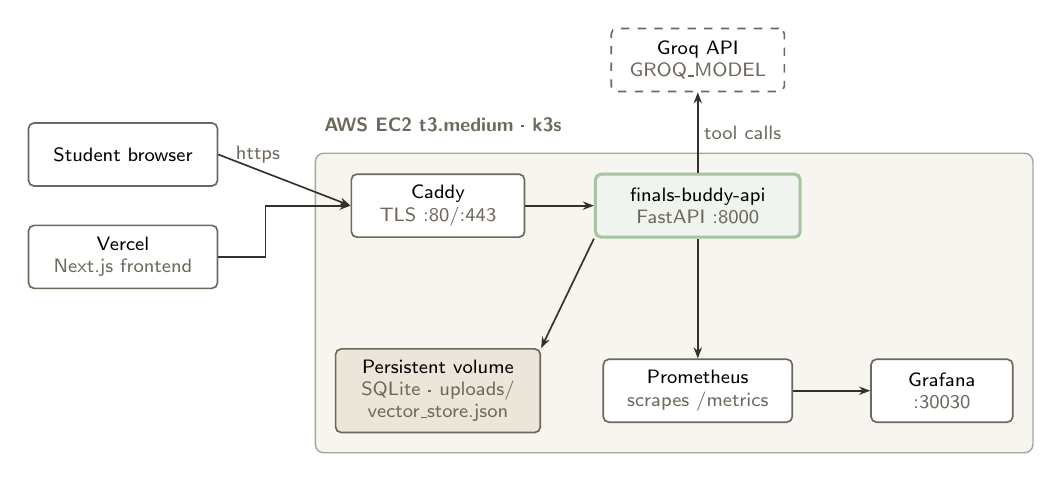
\begin{tikzpicture}[x=1mm, y=1mm]

% --- clients (outside the cluster) ---
\node[node, minimum width=24mm] (browser) at (0,0) {Student browser};
\node[node, minimum width=24mm] (vercel) at (0,-13) {Vercel\\\textcolor{fbMute}{Next.js frontend}};

% --- cluster contents ---
\node[node, minimum width=22mm] (caddy) at (40,-6.5) {Caddy\\\textcolor{fbMute}{TLS :80/:443}};
\node[accent, minimum width=26mm] (api) at (73,-6.5) {finals-buddy-api\\\textcolor{fbMute}{FastAPI :8000}};
\node[store, minimum width=26mm] (vol) at (40,-30) {Persistent volume\\\textcolor{fbMute}{SQLite · uploads/}\\\textcolor{fbMute}{vector\_store.json}};
\node[node, minimum width=24mm] (prom) at (73,-30) {Prometheus\\\textcolor{fbMute}{scrapes /metrics}};
\node[node, minimum width=18mm] (graf) at (104,-30) {Grafana\\\textcolor{fbMute}{:30030}};

% --- external dependency ---
\node[ext, minimum width=22mm] (groq) at (73,12) {Groq API\\\textcolor{fbMute}{GROQ\_MODEL}};

% --- cluster boundary, label placed outside so nothing is obscured ---
\begin{scope}[on background layer]
  \node[grp, fit=(caddy)(api)(vol)(prom)(graf)] (cluster) {};
\end{scope}
\node[grplabel, anchor=south west] at ([shift={(0,1.5mm)}]cluster.north west)
  {AWS EC2 t3.medium · k3s};

% --- edges ---
\draw[flow] (browser.east) -- node[flowlabel, above, pos=0.3]{https} (caddy.west);
\draw[flow] (vercel.east) -- ++(6,0) |- (caddy.west);
\draw[flow] (caddy) -- (api);
\draw[flow] (api) -- node[flowlabel, right]{tool calls} (groq);
\draw[flow] (api) -- (prom);
\draw[flow] (prom) -- (graf);
\draw[flow] (api.south west) -- (vol.north east);

\end{tikzpicture}
\caption{One EC2 node runs the API, its TLS front door, and its own monitoring.
Only ports 80 and 443 are public; Grafana is restricted to the operator's IP.}
\end{figure}

The backend is deliberately self-contained: SQLite for relational data, a
file-backed TF-IDF vector store for RAG (no external vector DB), and Groq as the
only external AI dependency. Everything that must survive a redeploy lives on the
one persistent volume.

The environment is described in Terraform (\code{infra/}), and deployments
arrive through GitHub Actions over AWS Systems Manager --- there is no SSH key
and port 22 is closed.

% ─────────────────────────────────────────────────────────────────────────────
\section{Tech stack}

\begin{tabularx}{\textwidth}{>{\bfseries}l L}
\toprule
\rowcolor{fbBrown}\hdr{Layer} & \hdr{Technology} \\
\midrule
Frontend        & Next.js 16, React 19, TypeScript 5, Tailwind CSS 4 \\
Rich editor     & TipTap 3 (+ math extension, KaTeX) \\
Icons           & lucide-react \\
Backend         & FastAPI, Uvicorn, Python 3.12 \\
ORM / DB        & SQLAlchemy 2, SQLite \\
LLM             & Groq, model set by \code{GROQ\_MODEL} (default
                  \code{qwen/qwen3.8-27b}) via groq SDK + LangChain \\
Agent loop      & LangChain / langchain-groq \\
RAG retrieval   & Custom local TF-IDF cosine store (\code{vector\_store.py}) \\
Doc parsing     & pypdf, docx2txt, python-pptx \\
Crypto          & \code{cryptography} (Fernet) for BYOK key encryption \\
Metrics         & prometheus-client (\code{app/observability.py}) \\
Orchestration   & k3s (single-node Kubernetes) \\
TLS             & Caddy, automatic Let's Encrypt \\
Monitoring      & Prometheus + Grafana, in-cluster \\
IaC             & Terraform (EC2, ECR, IAM, SSM Parameter Store) \\
CI/CD           & GitHub Actions, OIDC to AWS, deploy over SSM \\
Deploy          & Docker $\rightarrow$ ECR $\rightarrow$ k3s on AWS EC2;
                  frontend on Vercel \\
\bottomrule
\end{tabularx}

\begin{tcolorbox}[colback=fbCream,colframe=fbSage,boxrule=1pt,arc=2pt,left=8pt,right=8pt,top=6pt,bottom=6pt]
\textbf{Note on Next.js.} \code{frontend/AGENTS.md} warns this is a newer Next.js
with breaking changes vs.\ older conventions --- consult
\code{node\_modules/next/dist/docs/} before writing frontend code.
\end{tcolorbox}

% ─────────────────────────────────────────────────────────────────────────────
\section{Repository layout}

\begin{lstlisting}
finals-buddy/
|-- backend/
|   |-- app/
|   |   |-- main.py          # FastAPI app + all HTTP endpoints (~1700 lines)
|   |   |-- models.py        # SQLAlchemy ORM models (the data model)
|   |   |-- schemas.py       # Pydantic request/response schemas
|   |   |-- database.py      # engine, SessionLocal, get_db dependency
|   |   |-- config.py        # env config + runtime Groq-key overrides
|   |   |-- auth.py          # PBKDF2 hashing + HMAC bearer tokens
|   |   |-- key_context.py   # BYOK + free-trial gating (contextvar routing)
|   |   |-- admin.py         # /api/admin/* router
|   |   |-- errors.py        # AIServiceError
|   |   |-- observability.py # Prometheus metrics for the RAG/LLM layer
|   |   `-- services/
|   |       |-- agents.py         # LLM agents (summarize, quiz, exam, ...)
|   |       |-- langchain_chat.py # RAG tutor (Groq tool-calling loop)
|   |       `-- vector_store.py   # local TF-IDF vector store
|   |-- tests/
|   |   |-- test_rag_eval.py      # retrieval quality gate (golden set)
|   |   `-- test_observability.py # metrics recording + safety
|   |-- Dockerfile
|   `-- requirements.txt
|-- infra/
|   |-- terraform/           # EC2, ECR, IAM (OIDC), SSM parameters
|   |-- k8s/                 # app, Caddy, Prometheus, Grafana manifests
|   `-- scripts/             # apply-manifests, populate-secrets, seed-demo
|-- frontend/
|   `-- src/
|       |-- app/
|       |   |-- page.tsx              # home / subject list
|       |   |-- login/page.tsx
|       |   |-- admin/page.tsx
|       |   `-- subject/[id]/page.tsx # main study workspace (~3800 lines)
|       |-- components/               # AccountSettings, NotionEditor, Toast
|       `-- lib/api.ts                # typed API client + session handling
|-- docs/                             # screenshots + this document
`-- README.md
\end{lstlisting}

% ─────────────────────────────────────────────────────────────────────────────
\section{Data model}

All tables are defined in \code{backend/app/models.py}. \code{User} owns
\code{Subject}s; almost everything else hangs off \code{Subject} with
\code{ON DELETE CASCADE}.

\begin{figure}[H]
\centering
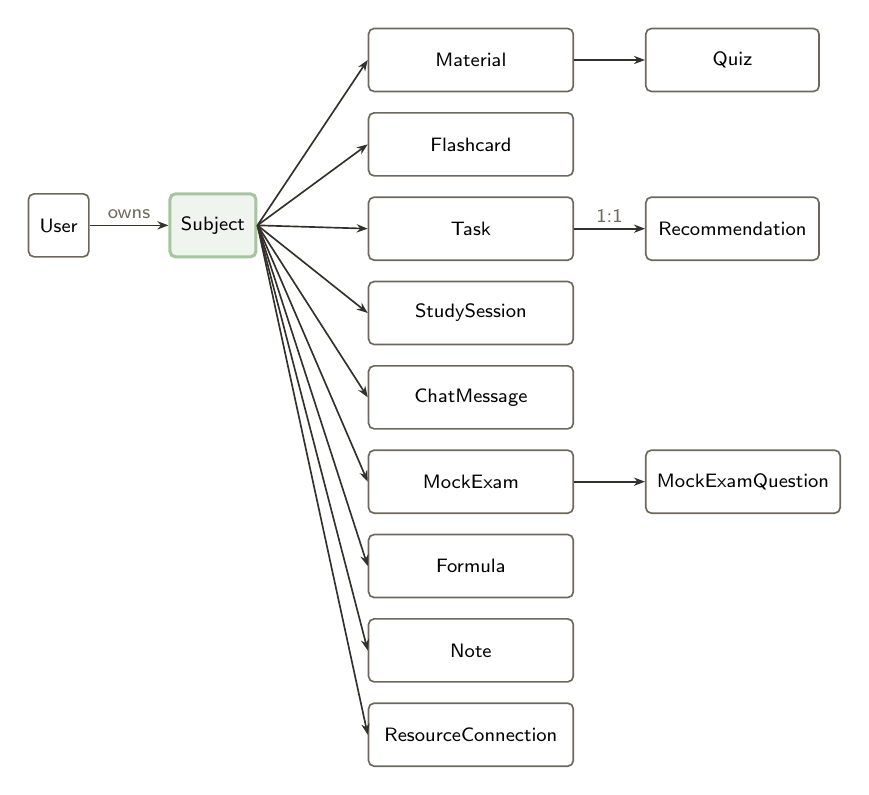
\begin{tikzpicture}

\node[node] (user) {User};
\node[accent, right=10mm of user] (subject) {Subject};

% children of subject, two columns
\node[node, right=14mm of subject, yshift=21mm, minimum width=26mm] (material) {Material};
\node[node, below=2.5mm of material, minimum width=26mm] (flash) {Flashcard};
\node[node, below=2.5mm of flash, minimum width=26mm] (task) {Task};
\node[node, below=2.5mm of task, minimum width=26mm] (session) {StudySession};
\node[node, below=2.5mm of session, minimum width=26mm] (chat) {ChatMessage};
\node[node, below=2.5mm of chat, minimum width=26mm] (exam) {MockExam};
\node[node, below=2.5mm of exam, minimum width=26mm] (formula) {Formula};
\node[node, below=2.5mm of formula, minimum width=26mm] (note) {Note};
\node[node, below=2.5mm of note, minimum width=26mm] (conn) {ResourceConnection};

% grandchildren
\node[node, right=9mm of material, minimum width=22mm] (quiz) {Quiz};
\node[node, right=9mm of task, minimum width=22mm] (rec) {Recommendation};
\node[node, right=9mm of exam, minimum width=22mm] (examq) {MockExamQuestion};

\draw[flow] (user) -- node[flowlabel, above]{owns} (subject);
\foreach \t in {material,flash,task,session,chat,exam,formula,note,conn}
  \draw[flow] (subject.east) -- (\t.west);

\draw[flow] (material) -- (quiz);
\draw[flow] (task) -- node[flowlabel, above]{1:1} (rec);
\draw[flow] (exam) -- (examq);

\end{tikzpicture}
\caption{\code{User} owns \code{Subject}; almost everything else hangs off
\code{Subject} with \code{ON DELETE CASCADE}.}
\end{figure}

Key fields worth knowing:

\begin{itemize}[leftmargin=1.4em]
\item \textbf{User} --- \code{groq\_api\_key\_encrypted} (Fernet-encrypted BYOK
  key, NULL = still on trial), \code{trial\_requests\_used} (counts free AI
  actions).
\item \textbf{Subject} --- \code{exam\_date}, \code{priority\_level} (1--5),
  \code{difficulty} (1--5), \code{confidence\_score} (0--100). These feed the
  recommendation formula.
\item \textbf{Material} --- \code{summary}, \code{key\_concepts} (JSON),
  \code{learning\_complexity}, \code{importance\_level},
  \code{deep\_research\_summary}.
\item \textbf{Flashcard} --- \code{box} (Leitner 1--5) + \code{next\_review\_date}
  drive spaced repetition.
\item \textbf{ResourceConnection} --- \code{source\_material\_id} $\rightarrow$
  \code{target\_material\_id} with a \code{connection\_type}
  (Prerequisite / Extension / Foundational): the AI-generated knowledge-map edges.
\end{itemize}

\subsection{Schema migrations}

There is no Alembic. On startup \code{main.py} runs
\code{Base.metadata.create\_all()} to create missing tables, followed by a series
of idempotent \code{ALTER TABLE ... ADD COLUMN} statements wrapped in try/except
(e.g.\ adding \code{deep\_research\_summary}, \code{groq\_api\_key\_encrypted},
\code{trial\_requests\_used}). This lightweight approach keeps the SQLite file
forward-compatible across redeploys without a migration tool.

% ─────────────────────────────────────────────────────────────────────────────
\section{Authentication}

\code{backend/app/auth.py}, intentionally dependency-free (hashlib / hmac /
secrets only):

\begin{itemize}[leftmargin=1.4em]
\item \textbf{Passwords:} PBKDF2-HMAC-SHA256, 260{,}000 iterations.
\item \textbf{Tokens:} \code{base64url(payload).hex(hmac\_sha256(secret, payload))},
  30-day TTL. Stateless --- no server session store.
\item \textbf{Secret:} \code{SECRET\_KEY} from env, else generated once and
  persisted to \code{.auth\_secret} next to the DB so sessions survive restarts.
\item \textbf{Frontend:} token + user cached in \code{localStorage}
  (\code{fb\_token} / \code{fb\_user}). \code{authFetch} in \code{lib/api.ts}
  attaches the bearer token and, on a 401, clears the session and redirects to
  \code{/login}.
\item \textbf{Admin:} \code{ADMIN\_EMAILS} env allowlist gates \code{/api/admin/*}.
  Single-owner project --- a plain email allowlist, no roles system.
\end{itemize}

% ─────────────────────────────────────────────────────────────────────────────
\section{AI agent layer}

\code{backend/app/services/agents.py}. Every agent calls \code{run\_llm()}, which
targets the Groq model named by \code{GROQ\_MODEL} at \code{temperature=0.3},
optionally in JSON mode, and raises \code{AIServiceError} on any failure rather
than fabricating content.

\begin{tcolorbox}[colback=fbCream,colframe=fbSage,boxrule=1pt,arc=2pt,left=8pt,right=8pt,top=6pt,bottom=6pt]
\textbf{Why the model is configuration.} It was hardcoded as
\code{llama-3.3-70b-versatile} in four places until Groq retired that model and
every AI feature began returning \code{404 model\_not\_found} at once. A single
\code{GROQ\_MODEL} setting means the next retirement is an environment variable,
not a code change. Any replacement must support native tool calling, which the
RAG tutor depends on; verify with a test call before switching.
\end{tcolorbox}

\begin{tabularx}{\textwidth}{>{\bfseries}l L}
\toprule
\rowcolor{fbBrown}\hdr{Agent} & \hdr{Job} \\
\midrule
SummarizationAgent & Exhaustive cited summary + key concepts + complexity /
  importance ratings (JSON). Emits Mermaid/ASCII diagrams and \code{[Slide N]}
  citations. \\
DeepResearchAgent & Under-the-hood mechanics, exam pitfalls, real-world case
  studies --- Markdown enrichment supplement. \\
QuizGenerationAgent & Flashcards + multiple-choice quizzes with mandatory source
  citations and per-question explanations; \code{generate\_more\_items} adds more
  while avoiding duplicates. \\
MockExamAgent & Generates 3 open-ended exam questions; grades typed answers 0--100
  on accuracy / completeness / terminology with constructive feedback. \\
FormulaExtractorAgent & Extracts formulas as LaTeX + variables + derivation steps
  (JSON). \\
CurriculumMapperAgent & Computes typed conceptual edges between materials
  $\rightarrow$ the knowledge map. \\
PlanningRecommendationAgent & \emph{Not an LLM call} --- deterministic Python
  scoring of tasks (see below). \\
\bottomrule
\end{tabularx}

\subsection{Recommendation score}

\code{PlanningRecommendationAgent.calculate\_recommendations} ranks pending tasks:

\begin{lstlisting}
score = (exam_urgency  * 0.4) + (topic_importance * 0.3)
      + (low_confidence * 0.2) + (incompletion    * 0.1)
\end{lstlisting}

Urgency is derived from days remaining to \code{exam\_date} ($\leq$1 day
$\rightarrow$ 10, decaying with distance); low-confidence from
\code{100 - confidence\_score}. The result is scaled to 0--100 for display. The
lowest-confidence topic with the nearest exam floats to the top.

% ─────────────────────────────────────────────────────────────────────────────
\section{Ingestion pipeline}

\code{POST /api/materials/upload} (\code{main.py}). Upload is a 7-step pipeline;
steps 1--2 run synchronously in the request, steps 3--7 run in a FastAPI
\code{BackgroundTask} so the HTTP response returns immediately with a
\code{job\_id}.

\begin{figure}[H]
\centering
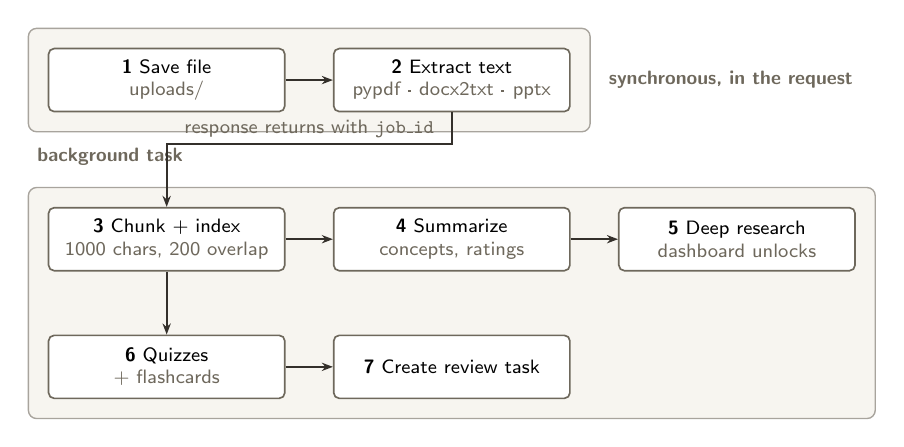
\begin{tikzpicture}[node distance=0pt]

\node[node, minimum width=30mm] (s1) {\textbf{1} Save file\\\textcolor{fbMute}{uploads/}};
\node[node, minimum width=30mm, right=6mm of s1] (s2) {\textbf{2} Extract text\\\textcolor{fbMute}{pypdf · docx2txt · pptx}};

\node[node, minimum width=30mm, below=12mm of s1] (s3) {\textbf{3} Chunk + index\\\textcolor{fbMute}{1000 chars, 200 overlap}};
\node[node, minimum width=30mm, right=6mm of s3] (s4) {\textbf{4} Summarize\\\textcolor{fbMute}{concepts, ratings}};
\node[node, minimum width=30mm, right=6mm of s4] (s5) {\textbf{5} Deep research\\\textcolor{fbMute}{dashboard unlocks}};

\node[node, minimum width=30mm, below=8mm of s3] (s6) {\textbf{6} Quizzes\\\textcolor{fbMute}{+ flashcards}};
\node[node, minimum width=30mm, right=6mm of s6] (s7) {\textbf{7} Create review task};

% boundaries
\begin{scope}[on background layer]
  \node[grp, fit=(s1)(s2)] (sync) {};
  \node[grp, fit=(s3)(s4)(s5)(s6)(s7)] (bg) {};
\end{scope}
\node[grplabel, anchor=west] at ([shift={(3pt,0)}]sync.east) {synchronous, in the request};
\node[grplabel, anchor=south west] at ([shift={(0,1.5mm)}]bg.north west) {background task};

\draw[flow] (s1) -- (s2);
\draw[flow] (s2.south) -- ++(0,-4mm) -| node[flowlabel, pos=0.25, above]{response returns with \texttt{job\_id}} (s3.north);
\draw[flow] (s3) -- (s4);
\draw[flow] (s4) -- (s5);
\draw[flow] (s3) -- (s6);
\draw[flow] (s6) -- (s7);

\end{tikzpicture}
\caption{Steps 1--2 run inside the request so the client gets a job id
immediately; the expensive AI work continues in the background and streams
progress over SSE.}
\end{figure}

Progress streams to the client over \textbf{Server-Sent Events} at
\code{GET /api/materials/upload-progress/\{job\_id\}}. The free-trial action is
consumed \emph{only after} the background pipeline succeeds, so a failed digestion
never burns a user's allowance.

Because the background thread runs after the response is sent, it cannot see the
request's contextvar; the resolved Groq key is passed explicitly and re-bound with
\code{set\_request\_key()} inside the thread (see \S\ref{sec:byok}).

% ─────────────────────────────────────────────────────────────────────────────
\section{RAG tutor}

\code{backend/app/services/langchain\_chat.py}, entered from
\code{POST /api/tutor/chat}.

\begin{figure}[H]
\centering
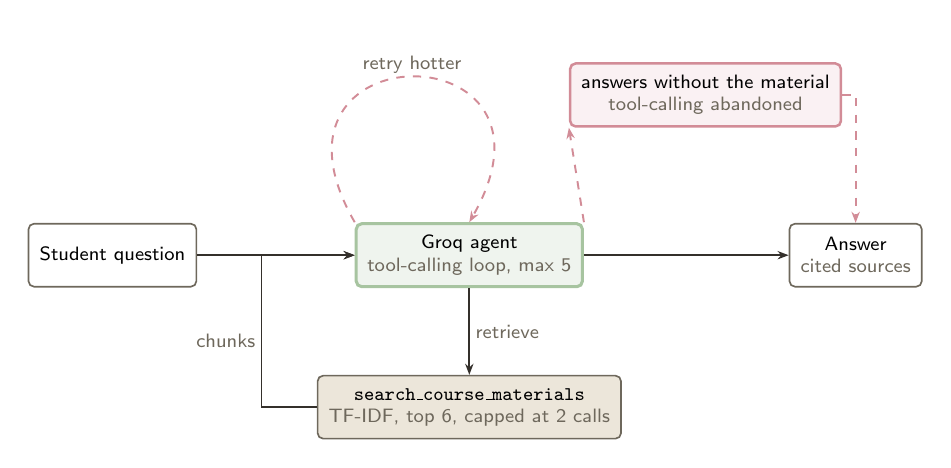
\begin{tikzpicture}

\node[node] (q) {Student question};
\node[accent, right=20mm of q] (llm) {Groq agent\\\textcolor{fbMute}{tool-calling loop, max 5}};
\node[node, right=26mm of llm] (ans) {Answer\\\textcolor{fbMute}{cited sources}};

\node[store, below=11mm of llm] (ret) {\texttt{search\_course\_materials}\\\textcolor{fbMute}{TF-IDF, top 6, capped at 2 calls}};

\node[degrade, above=12mm of llm, xshift=30mm] (notools)
  {answers without the material\\\textcolor{fbMute}{tool-calling abandoned}};

\draw[flow] (q) -- (llm);
\draw[flow] (llm) -- (ans);
\draw[flow] (llm.south) -- node[flowlabel, right]{retrieve} (ret.north);
\draw[flow] (ret.west) -- ++(-7mm,0) |- node[flowlabel, pos=0.22, left]{chunks} (llm.west);

% self-loop: malformed tool call is retried at a higher temperature
\draw[warn] (llm.north west) to[out=120, in=60, looseness=5]
  node[flowlabel, above, align=center, inner sep=1pt]{retry hotter} (llm.north);

% the silent path: give up on tools, still answer
\draw[warn] (llm.north east) -- (notools.south west);
\draw[warn] (notools.east) -| (ans.north);

\end{tikzpicture}
\caption{The two dashed paths still return a confident answer to the student.
The right-hand one answers without consulting their material at all, which is why
it is counted rather than merely logged.}
\end{figure}

\begin{itemize}[leftmargin=1.4em]
\item \textbf{Retrieval:} \code{vector\_store.py} is a from-scratch
  \textbf{TF-IDF cosine} store persisted as \code{vector\_store.json} --- no
  external vector DB, no embedding API. It computes IDF over the filtered document
  set at query time and returns the top-$k$ chunks. Documents are filtered by
  \code{subject\_id} so a query only ever sees the current subject's material.
\item \textbf{Agent loop:} a Groq tool-calling loop (max 5 iterations) with three
  tools --- \code{search\_course\_materials}, \code{get\_subject\_info},
  \code{get\_study\_progress}. Search is hard-capped at 2 calls per message.
\item \textbf{Payload size:} each retrieved chunk is capped at 800 characters,
  which is what bounds the context sent to Groq. An ONNX text compressor
  (Headroom) used to sit here; it was removed after measurement showed it was
  compressing nothing (see \S\ref{sec:observability}).
\item \textbf{Personas (\code{mode}):} \code{standard}, \code{simplified}
  (``explain like I'm 5''), and \code{analogies} inject different system-prompt
  suffixes.
\item \textbf{Resilience:} on a malformed tool call the loop retries at escalating
  temperature (greedy decoding would just reproduce the same bad call); if
  tool-calling can't be recovered it falls back to a direct no-tools answer. In
  trial mode only, a 429 rate-limit spills over to a second server key
  (\code{GROQ\_API\_KEY\_2}) --- a personal key never spills onto the owner's
  account.
\end{itemize}

\begin{tcolorbox}[colback=fbCream,colframe=fbSage,boxrule=1pt,arc=2pt,left=8pt,right=8pt,top=6pt,bottom=6pt]
\textbf{Every resilience path above is counted.} Each one still returns a
confident answer to the student, so none of them shows up as an error. A run that
falls back to a no-tools answer has stopped using the student's material
entirely while still looking healthy. The metrics in
\S\ref{sec:observability} exist to make those paths visible.
\end{tcolorbox}

% ─────────────────────────────────────────────────────────────────────────────
\section{BYOK + free-trial model}\label{sec:byok}

\code{backend/app/key\_context.py}. The app used to share one server Groq key for
every visitor; this module makes AI usage freemium so hosting cost stays flat.

\begin{itemize}[leftmargin=1.4em]
\item New accounts get \code{FREE\_TRIAL\_LIMIT = 5} AI actions on the
  \textbf{server} key.
\item After that, the user saves a personal Groq key (via
  \code{PUT /api/account/groq-key}), which is validated with a live
  \code{models.list()} call and stored \textbf{Fernet-encrypted} at rest. The
  Fernet key is derived (SHA-256) from the app's existing \code{SECRET\_KEY}, so
  there is no new secret to manage. Keys are never returned in full --- only a
  masked hint (\code{gsk\_...4f9a}).
\item \textbf{Key routing:} the resolved per-request key is stashed in a
  \code{contextvars.ContextVar}; \code{agents.run\_llm} and the tutor read it via
  \code{get\_current\_key()}. This threads a per-user key through module-level Groq
  client singletons without rewriting every agent signature. \code{contextvars}
  are per-thread/task, so it is safe under FastAPI's sync threadpool and async
  workers.
\item \textbf{Gate:} \code{ai\_action()} (context manager) resolves the key,
  enforces the cap (HTTP 402 when exhausted, 503 when no key exists), and
  increments the trial counter \emph{only} on success. \code{count=False} covers
  auto-fired paths like recommendations that should use a key but not consume the
  allowance.
\end{itemize}

\subsection{Runtime key overrides}

\code{config.py} supports a \code{.runtime\_overrides.env} file: the admin
dashboard's ``rotate Groq key'' feature writes here (in the persisted data volume)
instead of editing the container's real \code{.env}, so key changes survive
\code{docker rm} + redeploy without rebuilding the image.

% ─────────────────────────────────────────────────────────────────────────────
\section{HTTP API reference}

All routes are under \code{/api}. All except signup/login require a bearer token.
Ownership is enforced per subject (\code{own\_subject} / \code{assert\_owner}).

\subsection{Auth \& account}
\begin{tabularx}{\textwidth}{l l L}
\toprule
\rowcolor{fbBrown}\hdr{Method} & \hdr{Path} & \hdr{Purpose} \\
\midrule
POST   & \code{/auth/signup} & Register, returns token \\
POST   & \code{/auth/login}  & Log in, returns token \\
GET    & \code{/auth/me}     & Current user \\
GET    & \code{/account}     & Account + trial/key status \\
PUT    & \code{/account/groq-key} & Save/validate personal Groq key \\
DELETE & \code{/account/groq-key} & Remove personal key (back to trial) \\
\bottomrule
\end{tabularx}

\subsection{Subjects}
\begin{tabularx}{\textwidth}{l l L}
\toprule
\rowcolor{fbBrown}\hdr{Method} & \hdr{Path} & \hdr{Purpose} \\
\midrule
POST   & \code{/subjects}       & Create subject \\
GET    & \code{/subjects}       & List subjects \\
GET    & \code{/subjects/\{id\}} & Subject dashboard payload \\
PATCH  & \code{/subjects/\{id\}} & Update (exam date, priority, confidence...) \\
DELETE & \code{/subjects/\{id\}} & Delete (cascades) \\
\bottomrule
\end{tabularx}

\subsection{Materials \& knowledge map}
\begin{tabularx}{\textwidth}{l l L}
\toprule
\rowcolor{fbBrown}\hdr{Method} & \hdr{Path} & \hdr{Purpose} \\
\midrule
POST  & \code{/materials/upload} & Upload + start ingestion, returns \code{job\_id} \\
GET   & \code{/materials/upload-progress/\{job\_id\}} & SSE progress stream \\
GET   & \code{/subjects/\{id\}/materials} & List materials \\
PATCH/DELETE & \code{/materials/\{id\}} & Edit / delete material \\
POST  & \code{/subjects/\{id\}/generate-map} & Build knowledge-map edges \\
GET   & \code{/subjects/\{id\}/map} & Fetch nodes + edges \\
\bottomrule
\end{tabularx}

\subsection{Study aids}
\begin{tabularx}{\textwidth}{l l L}
\toprule
\rowcolor{fbBrown}\hdr{Method} & \hdr{Path} & \hdr{Purpose} \\
\midrule
GET/POST    & \code{/subjects/\{id\}/flashcards} & List / add flashcards \\
PUT/DELETE  & \code{/flashcards/\{id\}} & Edit / delete \\
POST        & \code{/flashcards/\{id\}/review} & Record review, advance Leitner box \\
GET/POST    & \code{/subjects/\{id\}/quizzes} & List / add quizzes \\
PUT/DELETE  & \code{/quizzes/\{id\}} & Edit / delete \\
POST        & \code{/quizzes/\{id\}/answer} & Submit answer, get grading \\
POST        & \code{/subjects/\{id\}/generate-more} & Generate more flashcards/quizzes \\
*           & \code{/subjects/\{id\}/mock-exams}, \code{/mock-exams/\{id\}} & Mock exams (CRUD) \\
POST        & \code{/mock-exams/\{id\}/submit} & Submit + auto-grade \\
GET/POST    & \code{/subjects/\{id\}/formulas}, \code{/formulas/generate} & Formula sheets \\
*           & \code{/formulas/\{id\}} & Edit / delete / annotate \\
\bottomrule
\end{tabularx}

\subsection{Tasks, sessions, notes, tutor, dashboard}
\begin{tabularx}{\textwidth}{l l L}
\toprule
\rowcolor{fbBrown}\hdr{Method} & \hdr{Path} & \hdr{Purpose} \\
\midrule
*     & \code{/tasks}, \code{/subjects/\{id\}/tasks}, \code{/tasks/\{id\}} & Planner tasks \\
*     & \code{/study-sessions}, \code{/subjects/\{id\}/sessions} & Focus sessions \\
*     & \code{/subjects/\{id\}/notes}, \code{/notes/\{id\}} & Rich notes \\
POST  & \code{/tutor/chat} & RAG tutor (query + persona mode) \\
*     & \code{/subjects/\{id\}/chats}, \code{/chats/\{id\}} & Tutor history \\
GET   & \code{/dashboard/recommendations} & Ranked next actions \\
GET   & \code{/dashboard/summary} & Aggregate stats \\
\bottomrule
\end{tabularx}

\subsection{Admin (\code{ADMIN\_EMAILS} only)}
\code{GET /admin/overview}, \code{GET /admin/logs}, \code{GET /admin/health},
\code{GET|PUT /admin/config} --- usage stats, app logs (from the stdout tee),
health checks, and live Groq-key rotation.

% ─────────────────────────────────────────────────────────────────────────────
\section{Frontend}

Next.js App Router. Three main routes:

\begin{itemize}[leftmargin=1.4em]
\item \textbf{\code{/} (page.tsx)} --- auth gate + subject list/creation.
\item \textbf{\code{/subject/[id]} (page.tsx, \textasciitilde 3800 lines)} --- the
  study workspace: dashboard, materials, flashcards, quizzes, mock exams, formula
  sheets, knowledge map, notes, tutor chat, focus mode. This is where most of the
  product lives.
\item \textbf{\code{/admin}} --- admin dashboard (usage, logs, health, key
  rotation).
\end{itemize}

\code{lib/api.ts} is the single typed API client: session helpers,
\code{authFetch} (bearer + 401 redirect), and \code{ApiError} (carries HTTP status
so callers can branch, e.g.\ 403 $\rightarrow$ ``not authorized''). \code{API\_BASE}
comes from \code{NEXT\_PUBLIC\_API\_URL} (defaults to
\code{http://127.0.0.1:8000/api}). Notes use the TipTap-based \code{NotionEditor}
with math/KaTeX support.

% ─────────────────────────────────────────────────────────────────────────────
\section{Observability}\label{sec:observability}

\code{backend/app/observability.py} defines every metric; they are exposed at
\code{GET /metrics} and scraped by Prometheus every 15 seconds. The existing code
was touched in four places only, each a single line or a thin wrapper.

The point is to measure the \emph{model}, not just the server. Uptime and CPU say
nothing about whether the tutor is still using the student's material.

\begin{tabularx}{\textwidth}{>{\ttfamily\small}l L}
\toprule
\rowcolor{fbBrown}\hdr{Metric} & \hdr{What it catches} \\
\midrule
fb\_llm\_no\_tools\_fallback\_total & The agent answered without the student's
  materials. Still a 200 response. \\
fb\_llm\_tool\_validation\_failures\_total & Groq rejected the model's tool call
  and it was retried hotter. \\
fb\_llm\_rate\_limit\_switch\_total & The primary key was exhausted and traffic
  moved to the backup. \\
fb\_llm\_search\_limit\_intercept\_total & The agent hit the hard two-search cap. \\
fb\_rag\_top1\_similarity & Best match score per query. A falling p50 means
  questions are drifting off-corpus. \\
fb\_rag\_zero\_match\_total & Nothing indexed for that subject at all. \\
fb\_rag\_empty\_result\_total & Material exists but nothing overlapped the
  question. Deliberately separate from the above. \\
fb\_rag\_payload\_tokens & Estimated context tokens per request. \\
fb\_llm\_duration\_seconds & End-to-end agent time, versus
  \code{fb\_rag\_query\_duration\_seconds} for retrieval alone. \\
fb\_tutor\_rolling\_satisfaction & Share of thumbs-up over the last 100 rated
  answers, fed by \code{POST /api/tutor/feedback}. \\
\bottomrule
\end{tabularx}

\subsection{Two rules the instrumentation follows}

\textbf{Metrics can never break a request.} Every recorder is wrapped in a
\code{safe()} decorator that swallows its own exceptions, with a test that feeds
deliberately malformed values into each one. A student must not get a 500 because
a histogram bucket was misconfigured.

\textbf{HTTP metrics label by route template, not path.}
\code{/api/subjects/41} and \code{/api/subjects/42} both report as
\code{/api/subjects/\{subject\_id\}}. Labelling by raw path mints a new time
series per subject id, which is the standard way to bury a Prometheus instance.

\subsection{What it found immediately}

Within the first hour of real traffic the metrics surfaced three live bugs that
logs, uptime and error rates had all missed:

\begin{enumerate}[leftmargin=1.6em]
\item \textbf{A retired model.} \code{llama-3.3-70b-versatile} returned
  \code{404 model\_not\_found}; every AI feature had been broken.
\item \textbf{A failover that had never worked.}
  \code{fb\_llm\_rate\_limit\_switch\_total} equalled the error count exactly:
  the primary key hit its limit, failed over to a backup key, and the backup
  returned 401. The failover made things worse, turning a retryable 429 into a
  hard auth error.
\item \textbf{A dependency doing nothing.} The ONNX text compressor could never
  initialise, because its model needs PyTorch and torch was deliberately excluded
  from the image. Measured at 0\,\% saving across every model and ratio. Removing
  it took the image from 1.31\,GB to 546\,MB.
\end{enumerate}

\subsection{Dashboard}

Grafana is provisioned from \code{infra/k8s/grafana-dashboard.json} with its
datasource wired automatically, so the dashboard exists on a fresh cluster with
no manual setup. Representative figures from the running system:

\begin{tabularx}{\textwidth}{>{\bfseries}l L}
\toprule
\rowcolor{fbBrown}\hdr{Measure} & \hdr{Value} \\
\midrule
Retrieval latency & 1.2\,ms \\
Full agent run & 4.0\,s average \\
Context per retrieval & $\approx$1{,}000 estimated tokens \\
Retrieval gate & precision@1 0.875, recall@3 1.000 \\
\bottomrule
\end{tabularx}

Retrieval is roughly four orders of magnitude faster than the model call, so all
perceived latency is the Groq round trip. Optimising the retriever would be
invisible to a student.

% ─────────────────────────────────────────────────────────────────────────────
\section{Testing}

\code{backend/tests/}, run by CI on every push.

\textbf{\code{test\_rag\_eval.py}} is a retrieval quality gate rather than a unit
test. Eight fixed questions each name the chunk that should rank first, scored
against a small committed corpus. The build fails below precision@1 0.75 or
recall@3 0.875. The corpus is synthetic on purpose: evaluating against the live
vector store would make the expected answers move whenever a student uploads a
file, and a test whose expected answer drifts is not a test.

It also guards three invariants: a student must never retrieve another subject's
material, an off-topic question must not produce a confident match, and an empty
corpus must return nothing rather than erroring.

\textbf{\code{test\_observability.py}} covers metric recording, including the
rule that a malformed value must never raise.

CI installs only numpy and prometheus-client for these, not the full requirements
file, so the gate finishes in seconds instead of waiting on unrelated
dependencies.

% ─────────────────────────────────────────────────────────────────────────────
\section{Configuration}

Backend env (\code{backend/.env}, see \code{.env.example}):

\begin{tabularx}{\textwidth}{>{\ttfamily}l L}
\toprule
\rowcolor{fbBrown}\hdr{Var} & \hdr{Purpose} \\
\midrule
GROQ\_API\_KEY   & Server key for the free trial \\
GROQ\_API\_KEY\_2 & Rate-limit fallback (trial mode only) \\
GROQ\_MODEL      & Groq model id, default \code{qwen/qwen3.8-27b}. Must support
                   native tool calling \\
DATABASE\_URL    & Defaults to \code{sqlite:///./finals\_buddy.db} \\
SECRET\_KEY      & Token signing + BYOK encryption seed (auto-generated if unset) \\
CORS\_ORIGINS    & Comma-separated allowed frontend origins \\
ADMIN\_EMAILS    & Comma-separated admin allowlist \\
RUNTIME\_OVERRIDES\_PATH & Path to the runtime key-override file \\
PORT / HOST      & Server bind (default \code{0.0.0.0:8000}) \\
\bottomrule
\end{tabularx}

Frontend env: \code{NEXT\_PUBLIC\_API\_URL} $\rightarrow$ backend \code{/api} base.

% ─────────────────────────────────────────────────────────────────────────────
\section{Running locally}

\textbf{Backend:}
\begin{lstlisting}
cd backend
python -m venv .venv && source .venv/bin/activate   # Windows: .venv\Scripts\activate
pip install -r requirements.txt
cp .env.example .env        # add GROQ_API_KEY
python -m uvicorn app.main:app --reload --port 8000
\end{lstlisting}
API docs (Swagger) at \code{http://127.0.0.1:8000/docs}.

\textbf{Frontend:}
\begin{lstlisting}
cd frontend
npm install
# .env.local: NEXT_PUBLIC_API_URL=http://127.0.0.1:8000/api
npm run dev        # http://localhost:3000
\end{lstlisting}

% ─────────────────────────────────────────────────────────────────────────────
\section{Deployment}

\begin{itemize}[leftmargin=1.4em]
\item \textbf{Backend:} Docker image (\code{backend/Dockerfile}),
  \code{python:3.12-slim}, architecture-agnostic across x86\_64 and ARM64. The
  app \emph{runs from} \code{/srv/finals-buddy/data} (its \code{WORKDIR}) while
  code lives at \code{/srv/finals-buddy}, so every relative artifact ---
  \code{finals\_buddy.db}, \code{uploads/}, \code{vector\_store.json},
  \code{.auth\_secret}, \code{.runtime\_overrides.env}, \code{logs/app.log} ---
  lands in one mountable volume:
\begin{lstlisting}
docker run -v finals_data:/srv/finals-buddy/data --env-file .env \
           -p 8000:8000 finals-buddy
\end{lstlisting}
  Uvicorn runs with \code{--proxy-headers --forwarded-allow-ips=*} behind a
  reverse proxy.
\item \textbf{Frontend:} Vercel; \code{NEXT\_PUBLIC\_API\_URL} points at the
  deployed backend.
\item \textbf{Logs:} stdout/stderr are teed to \code{logs/app.log} (size-capped)
  so the admin dashboard can show \code{docker logs}-equivalent output without
  mounting the Docker socket into the container.
\end{itemize}

\subsection{Infrastructure as code}

\code{infra/terraform/} describes the whole environment: an EC2 instance running
k3s, an ECR repository, IAM roles, and SSM parameters for secrets. The notable
choices:

\begin{itemize}[leftmargin=1.4em]
\item \textbf{k3s on one EC2 instance, not EKS.} The EKS control plane costs
  \$0.10/hour regardless of load. A single-node k3s cluster gives the same
  Kubernetes API and the same manifests for the price of the instance. This is
  not high availability and does not pretend to be; what it buys is declared
  state, health probes, rolling image updates and one-command rollback.
\item \textbf{No SSH key, port 22 closed.} Deploys and any manual access go
  through AWS Systems Manager, authenticated by IAM. There is no private key to
  store in GitHub.
\item \textbf{Secrets in SSM Parameter Store, encrypted.} Terraform creates each
  parameter with a placeholder and then ignores its value permanently via
  \code{lifecycle \{ ignore\_changes = [value] \}}. Real values are written out of
  band by \code{infra/scripts/populate-secrets.sh}, which pipes them straight
  into the AWS CLI without echoing them. No key reaches git or Terraform state,
  and rotating one no longer requires editing a file on a server.
\item \textbf{Local Terraform state.} Remote state with locking solves concurrent
  applies by multiple operators. There is one operator.
\end{itemize}

A \code{systemd} timer on the instance refreshes the ECR pull token (which
expires every 12 hours) and re-syncs secrets from SSM into a Kubernetes secret.

\subsection{Kubernetes}

\code{infra/k8s/} holds four workloads: the API, Caddy, Prometheus and Grafana.
Two decisions are specific to this app:

\begin{itemize}[leftmargin=1.4em]
\item \textbf{A persistent volume, because the app is stateful.} The backend
  writes \code{finals\_buddy.db}, \code{uploads/} and \code{vector\_store.json}
  into its working directory. Without the volume, every pod restart would wipe a
  student's materials and the entire retrieval corpus.
\item \textbf{Strategy is \code{Recreate}, not \code{RollingUpdate}.} SQLite on a
  \code{ReadWriteOnce} volume tolerates exactly one writer, and a rolling update
  briefly runs two pods. That trades a few seconds of downtime for not corrupting
  the database. It is a consequence of SQLite; moving to Postgres would remove it.
\end{itemize}

Caddy terminates TLS for the public hostname and obtains Let's Encrypt
certificates automatically, with its certificate store on its own volume so a
restart does not re-request them and trip rate limits. A plain-HTTP catch-all
block lets the pipeline smoke-test the instance by IP before DNS points at it.

\subsection{CI/CD}

\code{.github/workflows/ci-cd.yml}. A push to \code{master} is the only path to
production; \code{workflow\_dispatch} can deploy from another branch to prove the
pipeline without merging.

\begin{figure}[H]
\centering
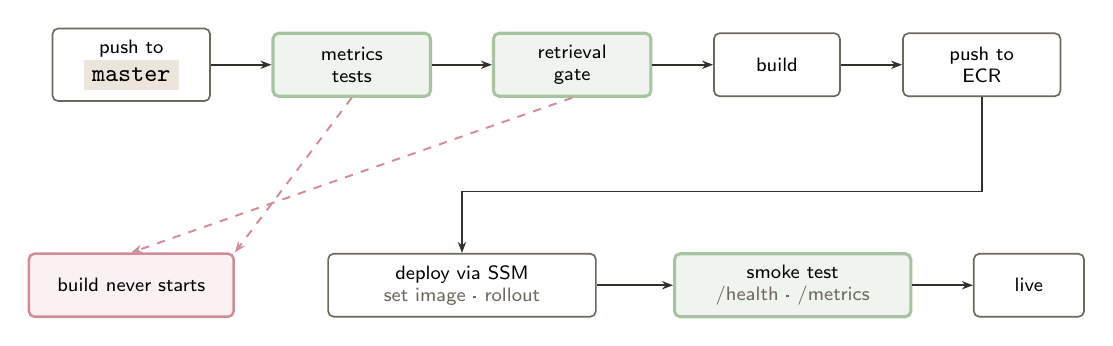
\begin{tikzpicture}[x=1mm, y=1mm]

\node[node, minimum width=20mm] (push)  at (0,0)   {push to\\\code{master}};
\node[accent, minimum width=20mm] (tests) at (28,0)  {metrics\\tests};
\node[accent, minimum width=20mm] (gate)  at (56,0)  {retrieval\\gate};
\node[node, minimum width=16mm] (build) at (82,0)  {build};
\node[node, minimum width=20mm] (ecr)   at (108,0) {push to\\ECR};

\node[node, minimum width=34mm] (deploy) at (42,-28) {deploy via SSM\\\textcolor{fbMute}{set image · rollout}};
\node[accent, minimum width=30mm] (smoke) at (84,-28) {smoke test\\\textcolor{fbMute}{/health · /metrics}};
\node[node, minimum width=14mm] (live)  at (114,-28) {live};

\node[degrade, minimum width=26mm] (stop) at (0,-28) {build never starts};

\draw[flow] (push) -- (tests);
\draw[flow] (tests) -- (gate);
\draw[flow] (gate) -- (build);
\draw[flow] (build) -- (ecr);
\draw[flow] (ecr.south) -- ++(0,-12) -| (deploy.north);
\draw[flow] (deploy) -- (smoke);
\draw[flow] (smoke) -- (live);

\draw[warn] (tests.south) -- (stop.north east);
\draw[warn] (gate.south) -- (stop.north);

\end{tikzpicture}
\caption{Two blocking gates sit before anything is built. A retrieval regression
fails the run while the only artefact is a test report.}
\end{figure}

GitHub authenticates to AWS through OIDC: each run receives a short-lived token,
and the trust policy accepts it only from this repository. No AWS credential is
stored in GitHub at all. The deploy role can push to one ECR repository and send
one SSM document to one instance, and nothing else.

\begin{figure}[H]
\centering
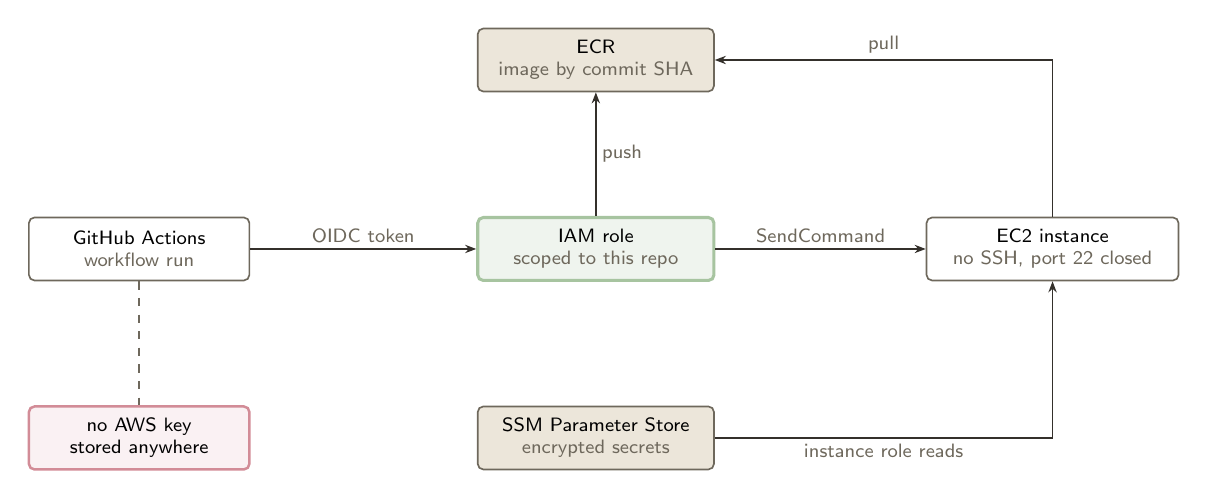
\begin{tikzpicture}[x=1mm, y=1mm]

\node[node, minimum width=28mm] (gha) at (0,0) {GitHub Actions\\\textcolor{fbMute}{workflow run}};
\node[accent, minimum width=30mm] (role) at (58,0) {IAM role\\\textcolor{fbMute}{scoped to this repo}};
\node[node, minimum width=32mm] (inst) at (116,0) {EC2 instance\\\textcolor{fbMute}{no SSH, port 22 closed}};

\node[store, minimum width=30mm] (ecr) at (58,24) {ECR\\\textcolor{fbMute}{image by commit SHA}};
\node[store, minimum width=30mm] (ssm) at (58,-24) {SSM Parameter Store\\\textcolor{fbMute}{encrypted secrets}};
\node[degrade, minimum width=28mm] (nokey) at (0,-24) {no AWS key\\stored anywhere};

\draw[flow] (gha.east) -- node[flowlabel, above, align=center]{OIDC token} (role.west);
\draw[flow] (role.east) -- node[flowlabel, above]{SendCommand} (inst.west);
\draw[flow] (role.north) -- node[flowlabel, right]{push} (ecr.south);
\draw[flow] (inst.north) |- node[flowlabel, pos=0.75, above]{pull} (ecr.east);
\draw[flow] (ssm.east) -| node[flowlabel, pos=0.25, below]{instance role reads} (inst.south);
\draw[dashed, draw=fbMute, line width=0.5pt] (gha.south) -- (nokey.north);

\end{tikzpicture}
\caption{The only thing GitHub holds is a role ARN. Secrets live encrypted in
SSM and are read by the instance itself, never passed through the pipeline.}
\end{figure}

\begin{tcolorbox}[colback=fbCream,colframe=fbSage,boxrule=1pt,arc=2pt,left=8pt,right=8pt,top=6pt,bottom=6pt]
\textbf{An IAM subtlety worth knowing.} \code{ssm:SendCommand} supports
resource-level permissions and is scoped to one instance and one document.
\code{ssm:GetCommandInvocation} does \emph{not} support them, so scoping it the
same way denies it outright and the pipeline fails after a successful deploy. It
has to be granted on \code{*}. Least privilege means knowing which actions can be
scoped, not narrowing every one of them reflexively.
\end{tcolorbox}

The smoke test checks \code{/metrics} as well as \code{/health}, because a deploy
that silently drops instrumentation leaves every dashboard flat, and flat reads
as quiet rather than broken.

The deployed image is tagged with the git commit SHA, so what is running traces
back to an exact commit with no manual build in the chain.

\subsection{Migration history}

The backend previously ran as a single Docker container on an Oracle Cloud
always-free VM, deployed by a GitHub Action holding a long-lived SSH key. That
box was a 1\,GB shape with under 500\,MiB free and already swapping, which could
not host k3s plus a monitoring stack without killing the application.

The move to AWS was performed as a DNS cutover: infrastructure, secrets,
pipeline, verification and seeding all happened while the old box still served
every user, and the only user-visible step was repointing one A record. The old
environment was left running throughout, so rollback was the same single record.

\begin{figure}[H]
\centering
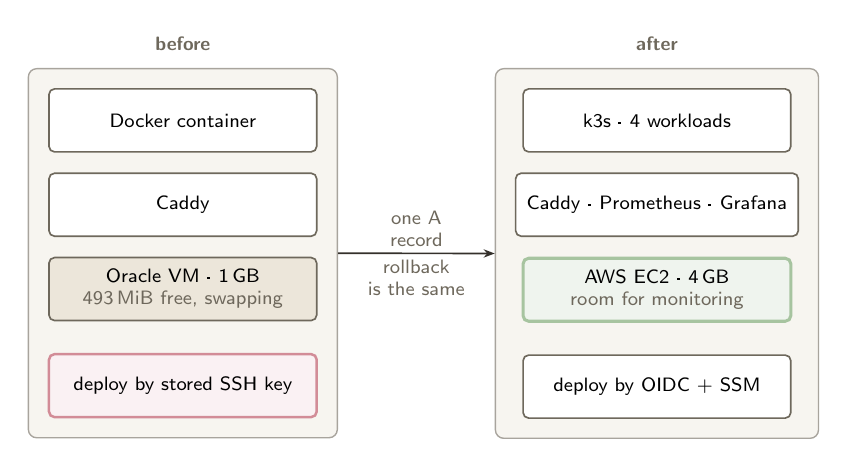
\begin{tikzpicture}

% before
\node[node, minimum width=34mm] (b1) {Docker container};
\node[node, below=2.5mm of b1, minimum width=34mm] (b2) {Caddy};
\node[store, below=2.5mm of b2, minimum width=34mm] (b3) {Oracle VM · 1\,GB\\\textcolor{fbMute}{493\,MiB free, swapping}};
\node[degrade, below=4mm of b3, minimum width=34mm] (b4) {deploy by stored SSH key};

% after
\node[node, right=26mm of b1, minimum width=34mm] (a1) {k3s · 4 workloads};
\node[node, below=2.5mm of a1, minimum width=34mm] (a2) {Caddy · Prometheus · Grafana};
\node[accent, below=2.5mm of a2, minimum width=34mm] (a3) {AWS EC2 · 4\,GB\\\textcolor{fbMute}{room for monitoring}};
\node[node, below=4mm of a3, minimum width=34mm] (a4) {deploy by OIDC + SSM};

\begin{scope}[on background layer]
  \node[grp, fit=(b1)(b2)(b3)(b4)] (bgrp) {};
  \node[grp, fit=(a1)(a2)(a3)(a4)] (agrp) {};
\end{scope}
\node[grplabel, above=1mm of bgrp] {before};
\node[grplabel, above=1mm of agrp] {after};

\draw[flow] (bgrp.east) -- node[flowlabel, above, align=center]{one A\\record}
  node[flowlabel, below, align=center]{rollback\\is the same} (agrp.west);

\end{tikzpicture}
\caption{The migration's only user-visible step, and its rollback, are the same
single DNS change.}
\end{figure}

For the original Oracle runbook see \code{DEPLOY.md} (not tracked in the public
repo); it is superseded by \code{infra/} but documents the manual path.

\vfill
\begin{center}
{\color{fbSage}\rule{0.4\textwidth}{1.5pt}}\\[0.4cm]
{\color{fbMute}\small Finals Buddy --- Technical Documentation}
\end{center}

\end{document}
